\documentclass{article}
\usepackage{amssymb}% http://ctan.org/pkg/amssymb
\usepackage{pifont}% http://ctan.org/pkg/pifont
\newcommand{\cmark}{\ding{51}}%
% Updated definition, see explanation below
\newcommand*{\fullref}[1]{\hyperref[{#1}]{\autoref*{#1} \nameref*{#1}}} % One single link
\usepackage{geometry}
\usepackage{parskip}
\usepackage{pdflscape}
\usepackage{lscape}
\usepackage[colorlinks,pdfpagelabels,pdfstartview = FitH,bookmarksnumbered = true,linkcolor = black,citecolor = black]{hyperref}		% Inhaltsverzeichnis anklickbar
\usepackage{scrpage2} 									% Kopf- und Fusszeile
\pagestyle{scrheadings}
\renewcommand{\headfont}{\small}
\ihead{
\includegraphics[width=3cm]{NTB-FHO_LOGO}} % Kopfzeile links
\setlength{\headsep}{18mm}
\ohead{xl2DB}												 % Kopfzeile rechts
\ifoot{} 													 % Fusszeile links
\cfoot{\thepage}					 							     % Fusszeile mitte
\ofoot{}													 % Fusszeile rechts
\setheadsepline{0.4pt}										 % fügt horizontale linie ein 
\usepackage[utf8]{inputenc}
\usepackage[T1]{fontenc}
\usepackage{color}
\usepackage{lmodern} % load a font with all the characters
\usepackage{graphicx}
\usepackage{caption}
\usepackage{subcaption}
\usepackage{enumitem}
\usepackage{titlesec}	
\setlist[description]{leftmargin=\parindent,labelindent=\parindent}
\graphicspath{{Bilder/}}
\geometry{
	a4paper,
	total={210mm,297mm},
	left=25mm,
	right=25mm,
	top=28mm,
	bottom=25mm
}
\definecolor{carrotorange}{rgb}{0.93, 0.57, 0.13}
\renewcommand{\contentsname}{Inhaltsverzeichnis}
\renewcommand{\listfigurename}{Abbildungsverzeichnis}
\renewcommand{\figurename}{Bild}
\hypersetup{urlcolor=blue}

%%%%%%%%%%%%%%%%%%%%%%%%%%% BEGIN %%%%%%%%%%%%%%%%%%%%%%%%%%%%%%%%%%

\begin{document}
\section*{\centering Bedienungsanleitung  - xl2DB}
\subsection*{Voraussetzungen}
Unsere Software benötigt die Microsoft Office Data Connectivity Components für die Datenbankfunktionen. Diese sind bei einer Installation von Microsoft Access > Version 2007 bereits dabei. Sollten Sie kein Microsoft Access installiert haben, können Sie diese Komponenten hier herunterladen und bitte installieren:

2007 Office System Driver: Data Connectivity Components:\\
\url{http://www.microsoft.com/en-us/download/details.aspx?id=23734}

\subsection*{Installation}
Für die Installation der Software muss man nur die Datei "setup.exe" ausführen die sich im Installations-Ordner befindet.

\subsection*{Excel File Vorbereitung}
Das Format des Excel Files muss wie in Bild 1. aufgebaut sein (ID, Anrede, Nachname etc.) und ist Case sensitiv (Gross/Kleinschreibung beachten): 
\begin{figure}[h]
	\begin{center}
		\centering
		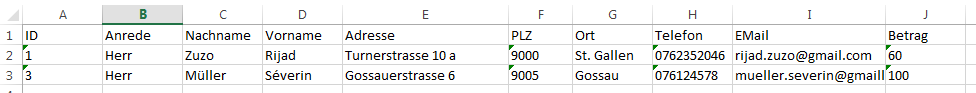
\includegraphics[width=0.8\paperwidth]{vorlageExcel}
		\caption{Excel Vorlage}
	\end{center}
\end{figure}

Auch muss das Blatt mit "Sheet1" beschriftet sein: 
\begin{figure}[h]
	\begin{center}
		\centering
		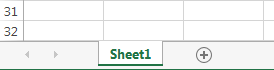
\includegraphics[width=0.3\paperwidth]{vorlageExcelSheet1}
		\caption{Excel Vorlage}
	\end{center}
\end{figure}

Dies sind Voraussetzungen für den reibungslosen Betrieb von xl2DB. Ohne diese Einstellungen funktioniert die Software nicht bzw. es ist mit Fehlern zu rechnen.
\newpage
\subsection*{Ausführung}
Nach erfolgreicher Installation wird die Software direkt ausgeführt und auf dem Desktop ist ein neues Icon mit dem Name xl2DB.exe zu finden.

\begin{figure}[h]
	\begin{center}
		\centering
		
\includegraphics[width=0.1\paperwidth]{Icon}
		\caption{xl2DB.exe Icon}
	\end{center}
\end{figure}

Beim ersten Aufruf der Applikation erscheint ein "Wilkommen" Fenster in welchem Sie hingewiesen werden, einen Datenbankpfad zu hinterlegen. Nach diesen Schritten ist die Software betriebsbereit.

\subsection*{Erste Schritte}
Beim ersten Aufruf der Applikation, muss via File - Choose Excel File, eine Datenbank geöffnet werden. Dieser wird intern gespeichert und beim nächsten Aufruf automatisch erneut aufgerufen, sofern die Datenbank noch vorhanden ist.

\begin{figure}[h]
	\begin{center}
		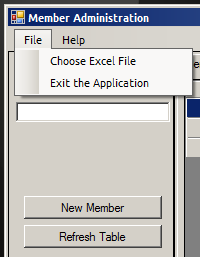
\includegraphics[width=0.2\paperwidth]{Pfads}
		\caption{Menü für die Auswahl eines Excel File}
	\end{center}
\end{figure}

Via File - Chose Excel File wird ein Dateibrowser geöffnet in dem Sie zum gewünschten File navigieren können:
\begin{figure}[h]
	\begin{center}
		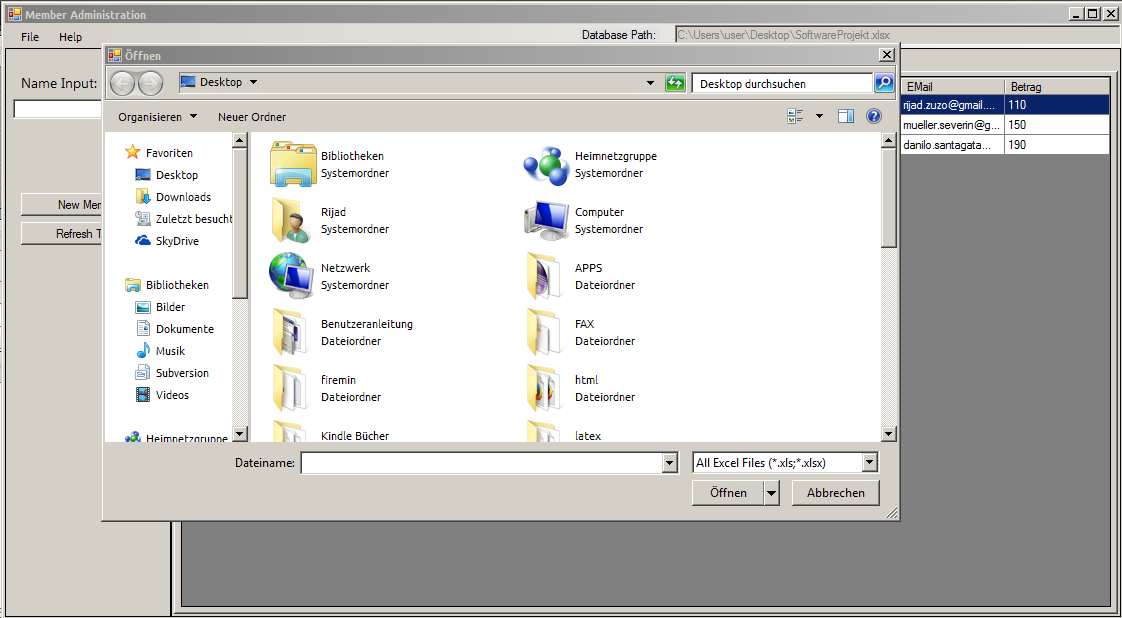
\includegraphics[width=0.8\paperwidth]{Filechooser}
		\caption{Dateibrowser}
	\end{center}
\end{figure}
\newpage
Sind Sie im gewünschten Pfad, kann das File durch einen Doppelklick oder markieren und einem Klick auf "Öffnen" geöffnet werden. Das Fenster schliesst sich und die Daten werden sofort ausgelesen und dargestellt:

\begin{figure}[h]
	\begin{center}
		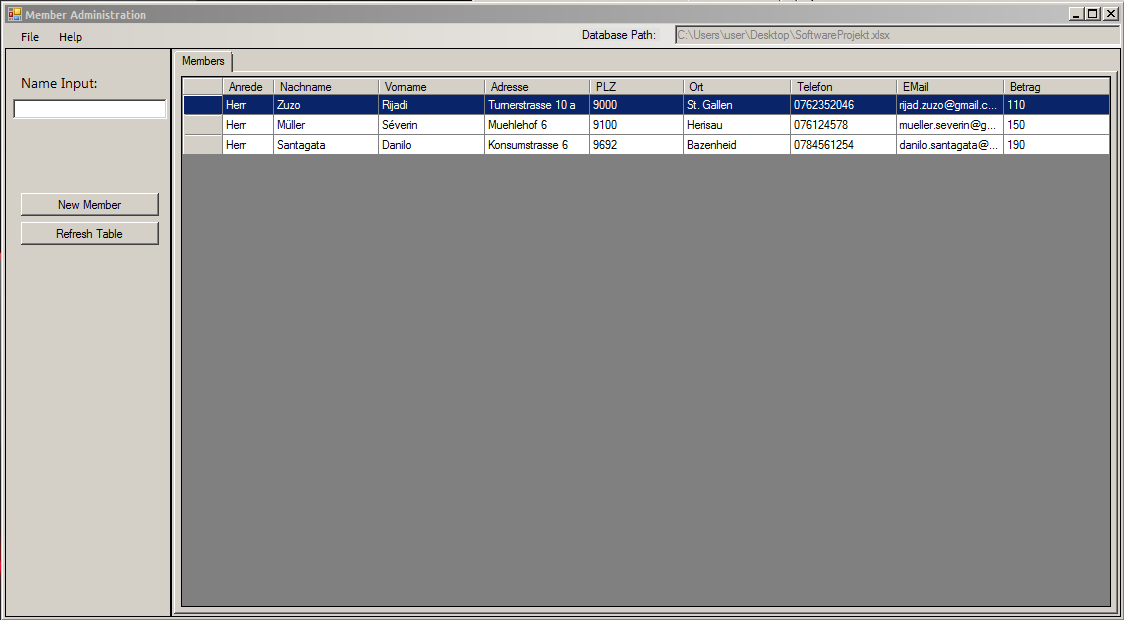
\includegraphics[width=0.8\paperwidth]{printscreen}
		\caption{Geladene Daten in Tabelle}
	\end{center}
\end{figure}

Sollte die Datei nicht geöffnet werden, überprüfen Sie den Pfad erneut mit File - Choose Excel File oder ob wie in Abschnitt "Excel File Vorbereitung" beschrieben, die Datei das gewünschte Format hat.

Die Software ist vollständig eingerichtet.

Bedienung: 
\begin{itemize}
\item Ein Klick auf "New Member" öffnet das Formular für die Eingabe eines neuen Mitgliedes (Bild 7.a).
 
\item Ein Klick in die Tabelle öffnet das "PersonWindow" mit allen Informationen zu einem Mitglied (Bild 7.b). Hier können auch Änderungen vorgenommen werden oder Mitglieder gelöscht werden.
\end{itemize}

 \begin{figure}[h]
 	\centering
 	\begin{subfigure}{.4\textwidth}
 		\centering
 		\includegraphics[width=.7\linewidth]{NewMemberGui}
 		\caption{Neues Mitglied Formular}
 		\label{fig:sub1}
 	\end{subfigure}%
 	\begin{subfigure}{.5\textwidth}
 		\centering
 		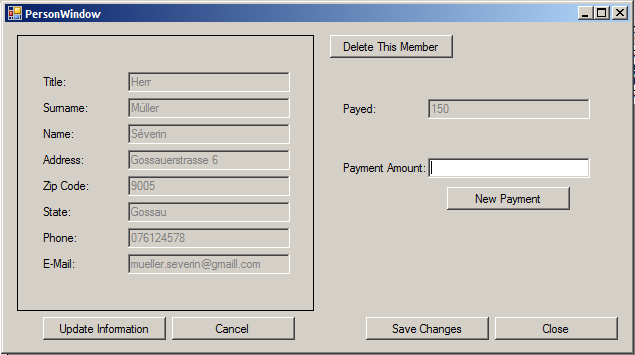
\includegraphics[width=.9\linewidth]{MemberInfoGUI}
 		\caption{Mitgliedsinformationen Fenster}
 		\label{fig:sub2}
 	\end{subfigure}
 	\caption{Fenster für weitere Details}
 	\label{fig:test}
 \end{figure}
 
 \centering \large Wir wünschen viel Spass und Erfolg bei der Nutzung unserer Software xl2DB. 
\end{document}